\documentclass[11pt,a4paper]{article}
% Shared preamble of the FEBAUTO Racing manuals.
\usepackage[margin=2.2cm,headheight=16pt]{geometry}
\usepackage[T1]{fontenc}
\usepackage{lmodern}
\usepackage{xcolor}
\usepackage{graphicx}
\usepackage{booktabs}
\usepackage{tabularx}
\usepackage{listings}
\usepackage{fancyhdr}
\usepackage{enumitem}
\usepackage{tikz}
\usetikzlibrary{arrows.meta}
\usepackage[hidelinks,colorlinks=true,linkcolor=febblue,urlcolor=febblue]{hyperref}

\definecolor{febblue}{HTML}{1C4687}
\definecolor{febgold}{HTML}{FDB515}
\definecolor{codebg}{HTML}{F3F4F6}

\lstset{
  basicstyle=\ttfamily\small,
  backgroundcolor=\color{codebg},
  frame=single, framerule=0pt, framesep=4pt,
  xleftmargin=4pt, xrightmargin=4pt,
  breaklines=true, columns=fullflexible, keepspaces=true,
  showstringspaces=false,
}
\newcommand{\file}[1]{\texttt{#1}}
\newcommand{\cmd}[1]{\texttt{#1}}
\newcommand{\rulebox}[1]{\par\noindent\colorbox{codebg}{\parbox{\dimexpr\linewidth-2\fboxsep}{#1}}\par\medskip}

\pagestyle{fancy}
\fancyhf{}
\fancyhead[L]{\color{febblue}\textbf{FEBAUTO Racing}}
\fancyhead[R]{\color{febblue}\nouppercase{\leftmark}}
\fancyfoot[C]{\thepage}
\renewcommand{\headrulewidth}{0.8pt}
\renewcommand{\headrule}{\color{febgold}\hrule width\headwidth height\headrulewidth}
\setcounter{tocdepth}{1}

% \febtitle{subtitle}{part lines}
\newcommand{\febtitle}[2]{%
\begin{titlepage}
  \centering
  \vspace*{2cm}
  
\includegraphics[width=5cm]{../../assets/feb_logo_512.png}\\[1.5cm]
  {\color{febblue}\Huge\bfseries FEBAUTO Racing}\\[6pt]
  {\Large #1}\\[2cm]
  \begin{tabular}{rl}#2\end{tabular}\\[3cm]
  Formula Electric at Berkeley\\
  September 2026, platform release v0.1.0\\[6pt]
  \url{https://github.com/FEBAutonomous/feb-racing}\\
  \url{https://febautonomous.github.io/feb-racing/}
\end{titlepage}
\tableofcontents
\newpage}

\usetikzlibrary{positioning,fit,backgrounds,calc}
\tikzset{
  box/.style={draw=febblue,thick,rounded corners=3pt,fill=white,align=center,inner sep=6pt,font=\small},
  soft/.style={draw=febblue!60,thick,rounded corners=3pt,fill=febblue!6,align=center,inner sep=6pt,font=\small},
  outer/.style={draw=febblue!40,dashed,rounded corners=6pt,inner sep=10pt},
  lbl/.style={font=\scriptsize\color{febblue},fill=white,inner sep=1pt},
  flow/.style={-{Stealth[length=6pt]},thick,febblue},
  both/.style={{Stealth[length=6pt]}-{Stealth[length=6pt]},thick,febblue},
}
\setlist{nosep,leftmargin=*}

\begin{document}
\pagestyle{fancy}
\fancyhead[R]{\color{febblue}Devkit v2 plan}

\begin{center}
  {\color{febblue}\LARGE\bfseries Devkit v2: a box of your own}\\[4pt]
  {\large How the development environment should work, on the laptop and on the car}\\[4pt]
  FEB autonomous team, 15 October 2026; built 16 October (\file{docs/devkit.md} is the how-to)
\end{center}
\medskip

\section*{The idea in four lines}
\begin{itemize}
  \item Every member gets a \textbf{persistent Linux box}: Ubuntu 22.04 with ROS 2 Humble, their own user, state that survives. It is a Docker container, but nobody types \cmd{docker}.
  \item \textbf{Everything robotic runs inside the box}: terminals, builds, bags, the bridge, the stack, the car's drivers.
  \item The \textbf{simulator and Foxglove are apps on the laptop}, opened like a game. They find the box on their own.
  \item The \textbf{same box runs on the Jetson}. Code that drives in the sim drives the car, untouched.
\end{itemize}

\section{On the laptop}

\begin{center}
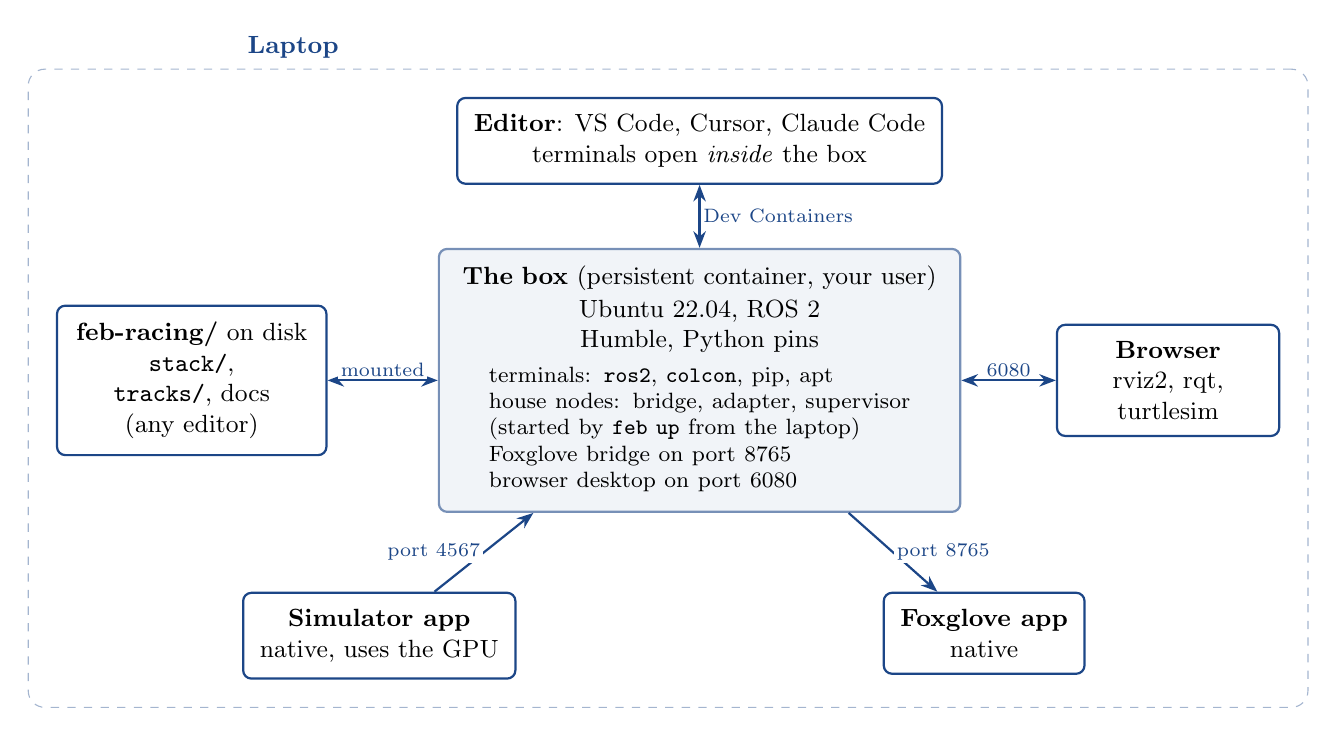
\begin{tikzpicture}[node distance=8mm, font=\small]
  \node[soft, text width=62mm] (box) {
    \textbf{The box} (persistent container, your user)\\[1pt]
    Ubuntu 22.04, ROS 2 Humble, Python pins\\[3pt]
    {\footnotesize\begin{tabular}{@{}l@{}}
      terminals: \cmd{ros2}, \cmd{colcon}, pip, apt\\
      house nodes: bridge, adapter, supervisor\\
      (started by \cmd{feb up} from the laptop)\\
      Foxglove bridge on port 8765\\
      browser desktop on port 6080
    \end{tabular}}};
  \node[box, above=of box] (editor) {\textbf{Editor}: VS Code, Cursor, Claude Code\\terminals open \emph{inside} the box};
  \node[box, left=14mm of box, text width=30mm] (files) {\textbf{feb-racing/} on disk\\\file{stack/}, \file{tracks/}, docs\\(any editor)};
  \node[box, right=12mm of box, text width=24mm] (web) {\textbf{Browser}\\rviz2, rqt,\\turtlesim};
  \node[box, below left=10mm and -10mm of box] (sim) {\textbf{Simulator app}\\native, uses the GPU};
  \node[box, below right=10mm and -10mm of box] (fox) {\textbf{Foxglove app}\\native};

  \draw[both] (files) -- node[lbl,above]{mounted} (box);
  \draw[both] (editor) -- node[lbl,right]{Dev Containers} (box);
  \draw[flow] (sim) -- node[lbl,left]{port 4567} (box);
  \draw[flow] (box) -- node[lbl,right]{port 8765} (fox);
  \draw[both] (box) -- node[lbl,above]{6080} (web);

  \begin{scope}[on background layer]
    \node[outer, fit=(files)(box)(editor)(sim)(fox)(web), label={[febblue,font=\small\bfseries]above left:Laptop}] {};
  \end{scope}
\end{tikzpicture}
\end{center}

What changed from today: the box is kept between sessions instead of rebuilt and deleted on every start; the editor's terminals are inside it; the sim is opened separately and finds the box; \cmd{feb-sim run} still exists as the one-shot race command.

\section{On the car}

\begin{center}
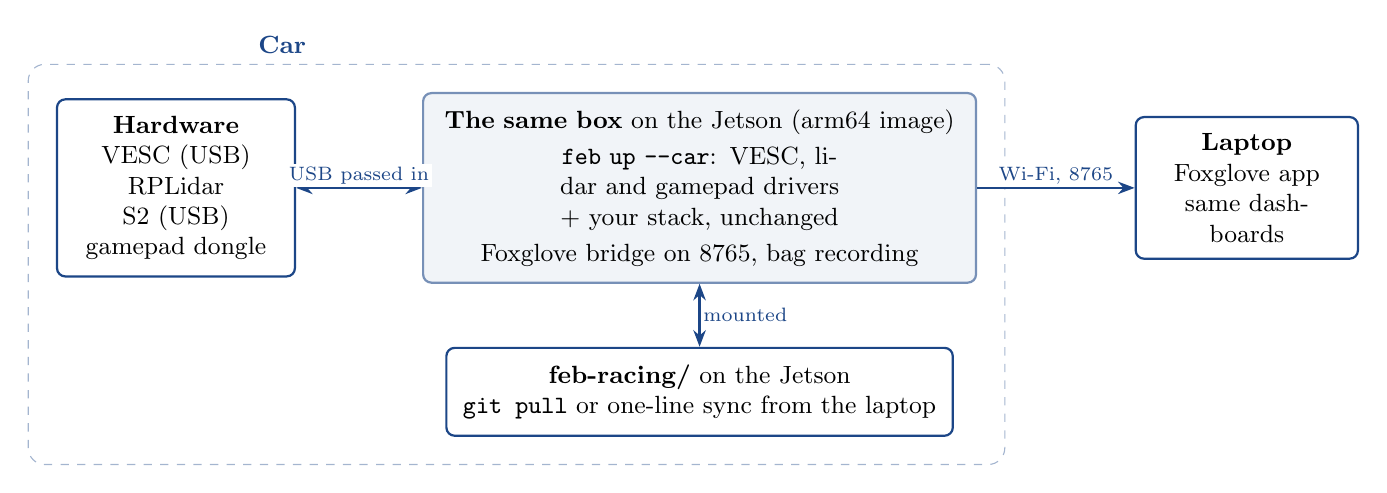
\begin{tikzpicture}[node distance=8mm]
  \node[soft, text width=66mm] (jbox) {
    \textbf{The same box} on the Jetson (arm64 image)\\[2pt]
    \cmd{feb up --car}: VESC, lidar and gamepad drivers\\ + your stack, unchanged\\[2pt]
    Foxglove bridge on 8765, bag recording};
  \node[box, left=16mm of jbox, text width=26mm] (hw) {\textbf{Hardware}\\VESC (USB)\\RPLidar S2 (USB)\\gamepad dongle};
  \node[box, right=20mm of jbox, text width=24mm] (lap) {\textbf{Laptop}\\Foxglove app\\same dashboards};
  \node[box, below=of jbox] (code) {\textbf{feb-racing/} on the Jetson\\\cmd{git pull} or one-line sync from the laptop};

  \draw[both] (hw) -- node[lbl,above]{USB passed in} (jbox);
  \draw[flow] (jbox) -- node[lbl,above]{Wi-Fi, 8765} (lap);
  \draw[both] (code) -- node[lbl,right]{mounted} (jbox);

  \begin{scope}[on background layer]
    \node[outer, fit=(hw)(jbox)(code), label={[febblue,font=\small\bfseries]above left:Car}] {};
  \end{scope}
\end{tikzpicture}
\end{center}

The only difference between laptop and car is what runs \emph{under} the stack: the sim bridge on the laptop, the real drivers on the Jetson. The stack never knows which.

\section{The contract that makes it one codebase}

A stack reads two topics and writes one, the RoboRacer standard:

\begin{center}
\begin{tabular}{lll}
\toprule
Topic & Type & Who publishes it \\
\midrule
\cmd{/scan} & LaserScan & sim adapter (laptop) or RPLidar driver (car) \\
\cmd{/odom} & Odometry & sim adapter or VESC driver \\
\cmd{/drive} & AckermannDriveStamped & \textbf{your stack}; sim adapter or VESC driver consumes it \\
\bottomrule
\end{tabular}
\end{center}

A small adapter node inside the box maps the simulator's \cmd{/autodrive/...} topics onto these. The current starter kit is moved onto the contract as the first user of it.

\section{The testing ladder}

\begin{center}
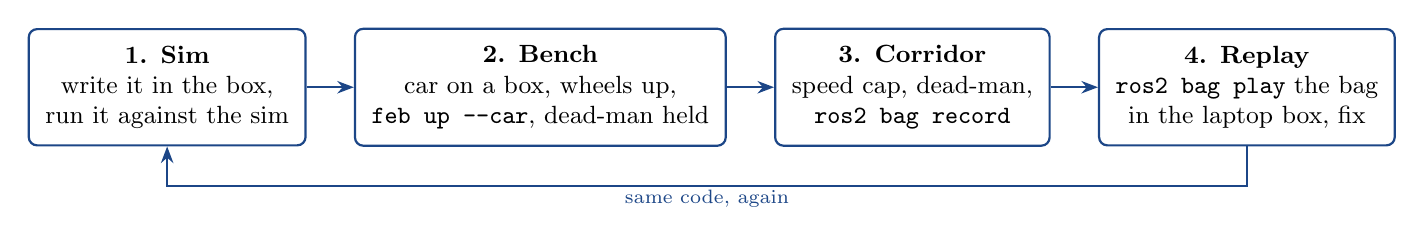
\begin{tikzpicture}[node distance=6mm]
  \node[box] (a) {\textbf{1. Sim}\\write it in the box,\\run it against the sim};
  \node[box, right=of a] (b) {\textbf{2. Bench}\\car on a box, wheels up,\\\cmd{feb up --car}, dead-man held};
  \node[box, right=of b] (c) {\textbf{3. Corridor}\\speed cap, dead-man,\\\cmd{ros2 bag record}};
  \node[box, right=of c] (d) {\textbf{4. Replay}\\\cmd{ros2 bag play} the bag\\in the laptop box, fix};
  \draw[flow] (a) -- (b); \draw[flow] (b) -- (c); \draw[flow] (c) -- (d);
  \draw[flow] (d.south) -- ++(0,-5mm) -| node[lbl,pos=0.25,below]{same code, again} (a.south);
\end{tikzpicture}
\end{center}

\section{A member's day, four ways}

\begin{description}[style=nextline]
  \item[Just a Linux box to mess around in (headless)] Open \file{feb-racing} in the editor, click \emph{Reopen in Container}. Every terminal is Ubuntu with ROS. Install things, write nodes, play bags. Close the editor, come back tomorrow, it is as you left it.
  \item[With a desktop (the onboarding lab)] Same box, gui flavour. One command puts a desktop in a browser tab for turtlesim, rqt\_graph and rviz2. Laggy but fine for teaching.
  \item[Racing in the sim] From a laptop terminal, \cmd{./feb up --track loop --driver feb\_driver}: house nodes, simulator and Foxglove in one go. Or start the house nodes by hand in a box terminal (\cmd{ros2 launch feb\_tools up.launch.py}) and double-click the simulator.
  \item[On the car] Put the code on the Jetson (\cmd{git pull}). \cmd{./feb up --car --driver my\_driver --mode-name inspection}. Hold the dead-man. Foxglove on the laptop at the Jetson's address.
\end{description}

\section{Today and proposed, side by side}

\begin{center}
\begin{tabularx}{\linewidth}{lXX}
\toprule
 & Today & Proposed \\
\midrule
Container & created and deleted on every \cmd{feb-sim run} & one persistent box per clone, \cmd{feb-sim reset} wipes it \\
User inside & root; files come out root-owned on Linux & your user \\
Builds & full \cmd{colcon build} on every start, 120\,s deadline & incremental, no deadline \\
Installed packages & lost on stop & kept \\
Terminals & \cmd{./feb-sim shell} from a laptop terminal (the old launcher) & \cmd{./feb code}: editor terminals, already inside; \cmd{./feb shell} too \\
Starting the sim & launcher starts it & app you open, or the launcher, either order \\
Visualiser & browser desktop with rviz2 (optional Foxglove) & Foxglove app by default, browser desktop for the lab \\
Topics & simulator names, \cmd{/autodrive/roboracer\_1/...} & \cmd{/scan}, \cmd{/odom}, \cmd{/drive} via an adapter \\
The car & follow the RoboRacer guide natively, port code by hand & same box, \cmd{feb up --car} \\
Submissions, league, CI & Docker image from the devkit & unchanged \\
\bottomrule
\end{tabularx}
\end{center}

\section{What changed in the repo}

\begin{itemize}
  \item \file{feb} (was \file{feb-sim}): the box is a persistent named container; \cmd{up}, \cmd{shell}, \cmd{code}, \cmd{reset}, \cmd{logs}; \cmd{--ws}, \cmd{--driver}, \cmd{--mode-name}, \cmd{--car}.
  \item \file{devkit/Dockerfile}: user \cmd{feb}, sudo, node and the Claude CLI, the VESC driver, rplidar, joy, ackermann\_msgs, scipy and casadi. \file{box.sh} is the box's process; \file{feb-up} builds a workspace and launches the house layer.
  \item \file{devkit/feb\_tools}: \file{sim\_adapter.py} (the contract from the simulator), \file{up.launch.py} (the house layer, sim or car), \file{car.launch.py} and \file{config/car.yaml} (the RoboRacer drivers).
  \item \file{devkit/feb\_supervisor}: the state machine.
  \item \file{starter\_kit}: \cmd{feb\_driver} and \cmd{feb\_cone\_driver} on the contract; every package carries a \file{driver.yaml}.
  \item \file{docs/devkit.md} rewritten; the lab and the three competitor manuals updated.
\end{itemize}

\section{Decisions}

Files live on the laptop and are mounted in; VS Code is the standard editor and Cursor works too;
Foxglove is the daily visualiser, the browser desktop stays for the lab and the odd rviz session;
the box persists; \cmd{feb up} is the one-shot command; Docker Desktop is the engine, OrbStack
allowed on Mac. Settled while building: all of our commands live on the laptop side as \cmd{feb},
inside the box there is only ROS and one launch file; the Jetson keeps its own clone of the FEB
folder and is updated by \cmd{git pull}; the gui image is the box's image for everyone (one
download), the base image stays the league's. Drivers carry a \file{driver.yaml} with modes
(\cmd{inspection}, \cmd{trackdrive}, and whatever else the code does), and the supervisor is the
only on-car manager: it decides whose command reaches the wheels.

Not yet done: a hardware test of \cmd{feb up --car} (the Jetson is not flashed), and the
\cmd{feb\_cone\_racer} package still reads the simulator's topics directly.

\section{Why not a VM}

For the member, a VM and the box are the same thing: a Linux machine that keeps its state. The difference is the plumbing.

\begin{center}
\begin{tabularx}{\linewidth}{lXX}
\toprule
 & The box & A VM \\
\midrule
Starts in & a second & 30 to 60 s \\
RAM & what is running & 4 to 8 GB reserved \\
Disk & about 5 GB, shared image & 20 to 40 GB per person \\
Install & Docker Desktop, then \emph{Reopen in Container} & hypervisor, ISO, Ubuntu, ROS by hand; different per laptop type \\
Updating the base & \cmd{docker pull}, seconds & gigabytes again, or by hand \\
Apple Silicon & same image, arm64 built by CI & separate arm64 build; nobody ships one \\
Reaching the sim & done for you & port forwarding per member \\
Same as the car & yes & no, two environments \\
Submissions & it is the submission & still need Docker \\
Desktop & browser tab, laggy & native, nicer \\
\bottomrule
\end{tabularx}
\end{center}

The VM wins one row, the desktop, which Foxglove covers. Penn's course can recommend a VM because its simulator is a Python package that lives inside the VM; ours is a native GPU app that cannot. A VM recipe can still be published as an unsupported option for anyone who wants a full Ubuntu desktop; it changes nothing above.

\end{document}
